\documentclass[12pt,a4paper]{article}

% Fonts and encoding
\usepackage[T1]{fontenc}
\usepackage[utf8]{inputenc}
\usepackage{times}
\usepackage{mathptmx}

% Layout
\usepackage[a4paper,margin=2.5cm]{geometry}
\usepackage{setspace}
\linespread{1.08}
\usepackage{parskip}
\setlength{\parskip}{0.6em}
\setlength{\parindent}{0pt}

% Graphics and floats
\usepackage{graphicx}
\usepackage{float}
\usepackage{subcaption}
\usepackage{booktabs}
\usepackage{siunitx}
\usepackage{amsmath,amssymb}
\usepackage{hyperref}
\hypersetup{colorlinks=true,linkcolor=blue,citecolor=blue,urlcolor=blue}
\usepackage{enumitem}
\usepackage{longtable}
\usepackage{array}
\usepackage{ragged2e}
\usepackage{fancyhdr}
\usepackage{csvsimple}
\usepackage{tikz}
\usetikzlibrary{shapes.geometric, arrows.meta, positioning}
\tikzset{
  startstop/.style={rectangle, rounded corners, minimum width=3.2cm, minimum height=1.0cm, text centered, draw=black, fill=red!20},
  io/.style={trapezium, trapezium stretches=true, trapezium left angle=70, trapezium right angle=110, minimum width=4cm, minimum height=1.0cm, text centered, draw=black, fill=blue!20},
  process/.style={rectangle, minimum width=4cm, minimum height=1.0cm, text centered, text width=4.6cm, draw=black, fill=orange!20},
  decision/.style={diamond, aspect=2.2, text centered, draw=black, fill=green!20, inner sep=1.2pt},
  arrow/.style={thick,-{Stealth[length=2.2mm,width=2.0mm]}}
}
\begin{document}


\begin{figure}[H]
  \centering
  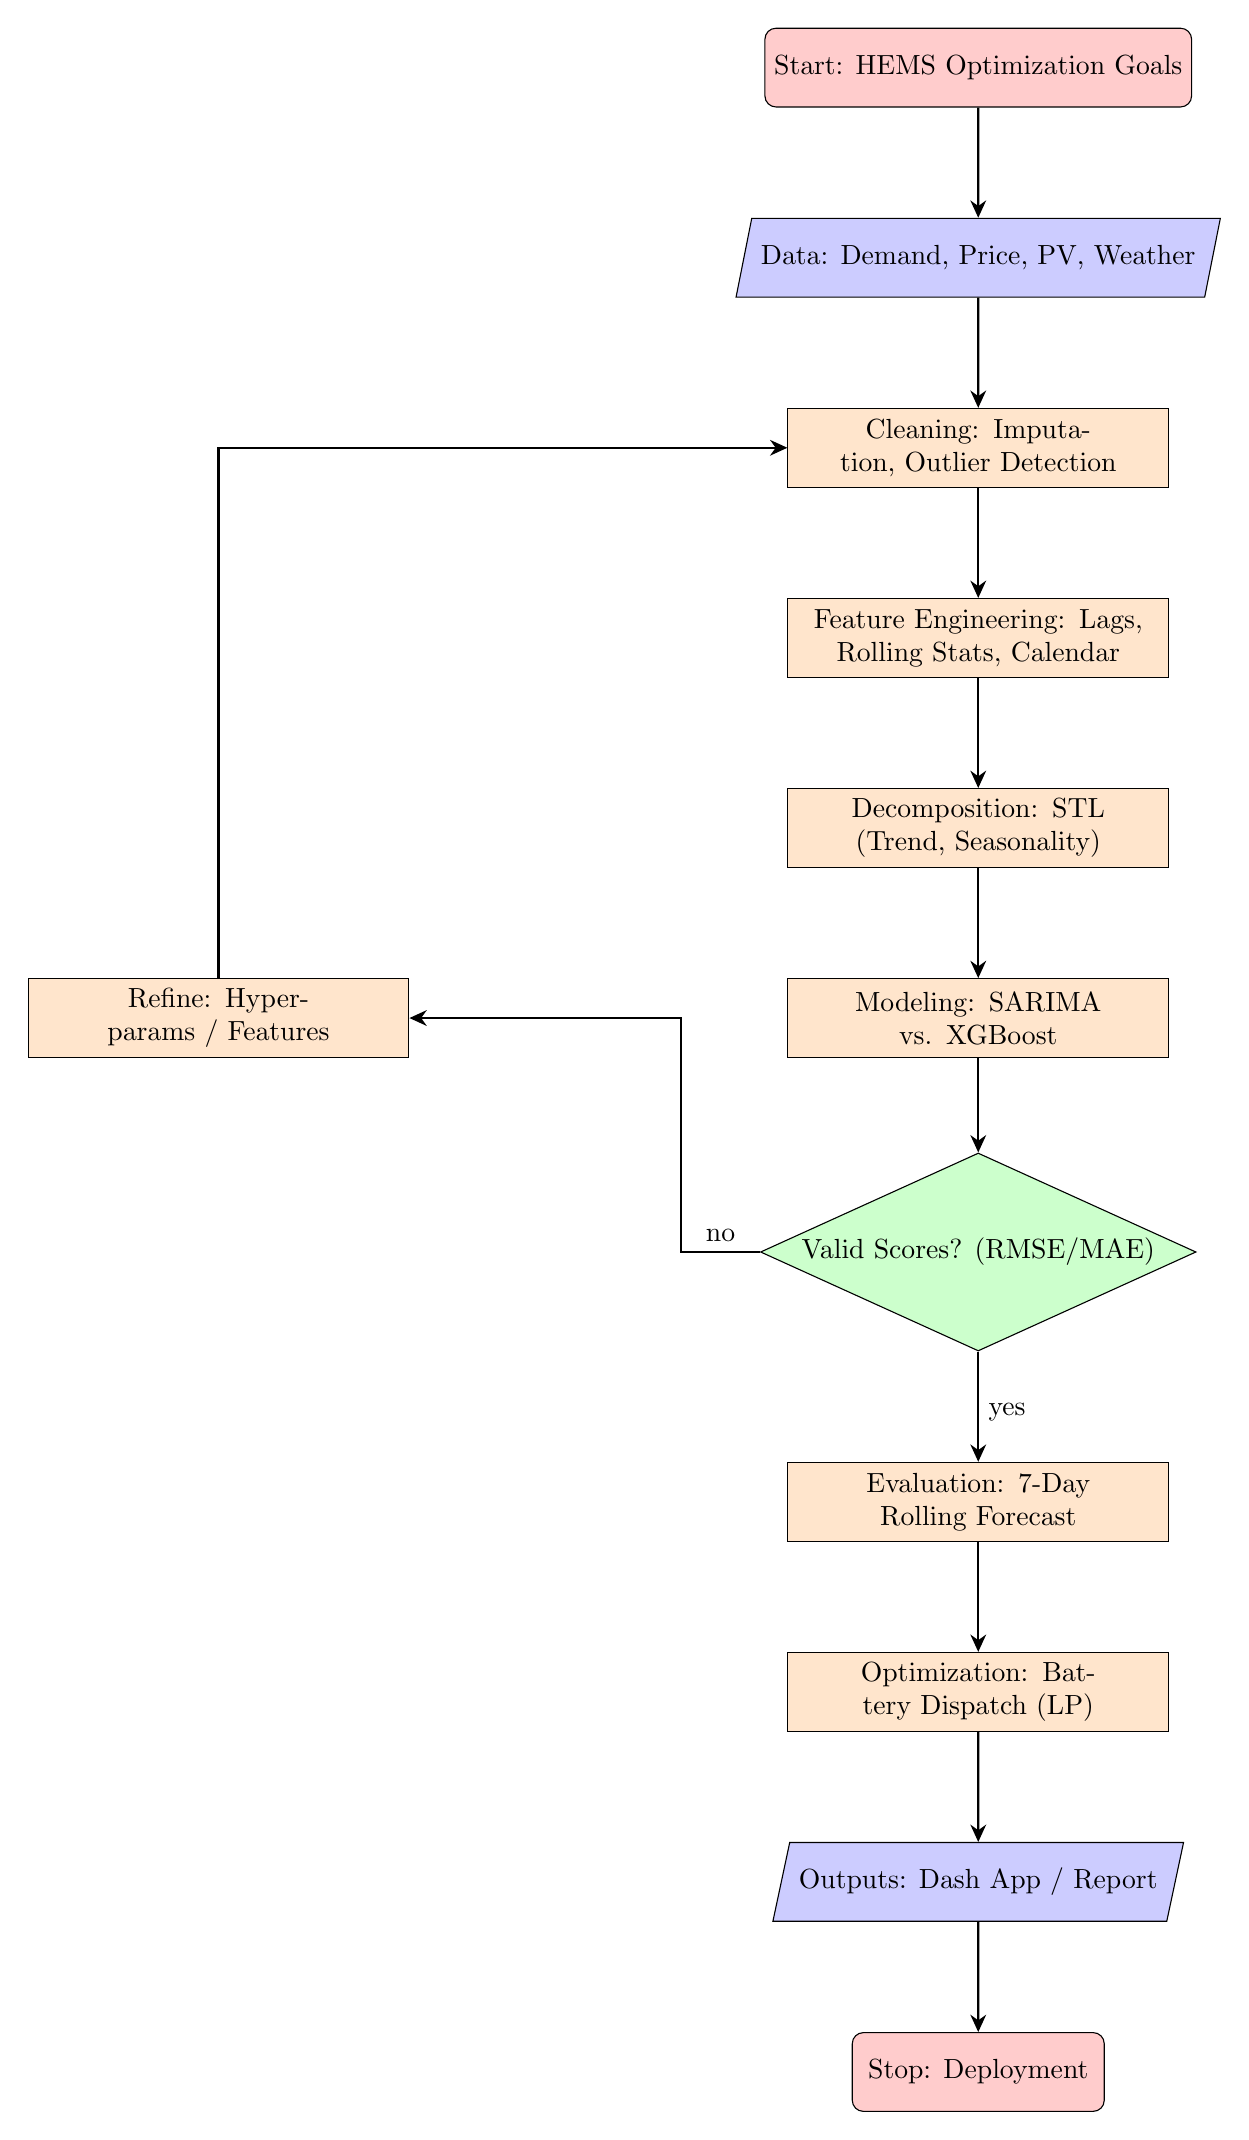
\begin{tikzpicture}[node distance=1.4cm]
    \node (start) [startstop] {Start: HEMS Optimization Goals};
    \node (data) [io, below=of start] {Data: Demand, Price, PV, Weather};
    \node (prep) [process, below=of data] {Cleaning: Imputation, Outlier Detection};
    \node (feat) [process, below=of prep] {Feature Engineering: Lags, Rolling Stats, Calendar};
    \node (decomp) [process, below=of feat] {Decomposition: STL (Trend, Seasonality)};
    \node (model) [process, below=of decomp] {Modeling: SARIMA vs. XGBoost};
    \node (dec) [decision, below=1.2cm of model] {Valid Scores? (RMSE/MAE)};
    \node (eval) [process, below=1.4cm of dec] {Evaluation: 7-Day Rolling Forecast};
    \node (opt) [process, below=of eval] {Optimization: Battery Dispatch (LP)};
    \node (out) [io, below=of opt] {Outputs: Dash App / Report};
    \node (stop) [startstop, below=of out] {Stop: Deployment};

    % forward arrows
    \draw[arrow] (start) -- (data);
    \draw[arrow] (data) -- (prep);
    \draw[arrow] (prep) -- (feat);
    \draw[arrow] (feat) -- (decomp);
    \draw[arrow] (decomp) -- (model);
    \draw[arrow] (model) -- (dec);
    \draw[arrow] (dec) -- node[right,pos=0.55]{yes} (eval);
    \draw[arrow] (eval) -- (opt);
    \draw[arrow] (opt) -- (out);
    \draw[arrow] (out) -- (stop);

    % feedback branch to avoid overlaps (route to the left)
    \node (fix) [process, left=4.8cm of model] {Refine: Hyperparams / Features};
    \draw[arrow] (dec.west) --++ (-1.0,0) node[above,pos=0.5]{no} |- (fix);
    \draw[arrow] (fix) |- (prep);
  \end{tikzpicture}
  \caption{Project plan (CRISP--DM: Understanding $\to$ Preparation $\to$ Modeling $\to$ Evaluation $\to$ Deployment). Clean layout avoids overlapping connectors.}
  \label{fig:lifecycle}
\end{figure}
\end{document}
